\documentclass[12pt]{article}
%\usepackage{geometry}                % See geometry.pdf to learn the layout options. There are lots.
%\geometry{letterpaper}                   % ... or a4paper or a5paper or ... 
%\geometry{landscape}                % Activate for for rotated page geometry
\usepackage[parfill]{parskip}    % Activate to begin paragraphs with an empty line rather than an indent
\usepackage{daves,fancyhdr,natbib,graphicx,dcolumn,amsmath,lastpage,url}
\usepackage{multicol}
\usepackage{amsmath,amssymb,epstopdf,longtable}
\usepackage[final]{pdfpages}
\usepackage{booktabs}

\DeclareGraphicsRule{.tif}{png}{.png}{`convert #1 `dirname #1`/`basename #1 .tif`.png}
\pagestyle{fancy}
\lhead{CE 5362 Surface Water Modeling}
\rhead{SPRING 2020}
\lfoot{}
\cfoot{}
\rfoot{Page \thepage\ of \pageref{LastPage}}
\renewcommand\headrulewidth{0pt}


\setcounter{MaxMatrixCols}{20}

%%%%%%%%%% Will's listing environment %%%%%%%
\usepackage[left=1.25in, right=1.25in,
            top=1in, bottom=1in]{geometry}                % See geometry.pdf to learn the layout options. There are lots.
\geometry{letterpaper}

\usepackage{ragged2e}

\usepackage{xcolor}
\newcommand{\codeRcolor}{0.93}
\newcommand{\codeGcolor}{0.93}
\newcommand{\codeBcolor}{0.93}
\definecolor{lightgrey}{rgb}{\codeRcolor,
                             \codeGcolor,
                             \codeBcolor}

\newcommand{\listingfont}{\fontsize{7pt}{8pt}\selectfont\ttfamily}
\usepackage{listings}
\lstset{basicstyle = \listingfont,
        breaklines = true,
        frame=tb,
        xleftmargin=12pt,
        framexleftmargin=6pt,
        framexrightmargin=6pt,
        xrightmargin=12pt,
        columns=fixed}
\lstset{lineskip=-1pt}
\lstset{backgroundcolor=\color{lightgrey}}


\usepackage[font={footnotesize},
            labelfont={sf,bf},
            textfont={sf},
            singlelinecheck=false,
            labelsep=none,
            justification=RaggedRight,
            aboveskip=0pt,
            belowskip=7pt plus 1pt minus 1pt,
            textformat=period]{caption}
\DeclareCaptionLabelSeparator{mystyle}{.\quad}
\captionsetup{labelsep=mystyle}
%%%%%%%%% End Will's listing environment ABOVE %%%%%%%%%

\begin{document}
\begingroup
\begin{center}
{\textbf{{CE 5362 Surface Water Modeling \\ Lesson 12}}}
\end{center}

\begin{center}
by \\
Theodore G. Cleveland \\%and Caroline M. Neale\\
Department of Civil, Environmental, and Construction Engineering\\
Texas Tech University\\
\end{center}

\begin{figure}[h!] %  figure placement: here, top, bottom, or page
\centering
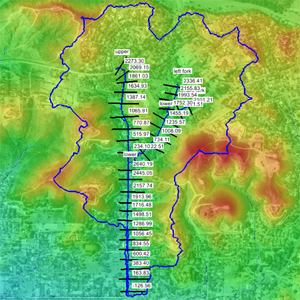
\includegraphics[width=5in]{hecras-med.png} 
\end{figure}

\endgroup
\tableofcontents
%%%%%%%%%%%%%%%%%%%%%%%%%%%%%%%%%%%%%%%
\section{HEC-RAS Confluence (Junctions)}
%%%%%%%%%%%%%%%%%%%%%%%%%%%
what is a junction?
how are they conceptualized?
options for simulation 

\subsection{Conceptualization}

\subsubsection{Tributary does not directly contribute momentum to main branch }

\subsubsection{Tribuitary directly contributes momentum to main branch}


\clearpage
\subsection{Examples}
\subsubsection{Example 1. -- using HEC-RAS Steady}

Figure  \ref{fig:confluence} is a sketch of a channel and tributary system with a road (bridge) crossing the main channel.  The cross sections are surveyed and the sections are included in Figure \ref{fig:cross-sections-table}

\begin{figure}[h!] %  figure placement: here, top, bottom, or page
   \centering
   \includegraphics[width=4.5in]{confluence.png} 
   \caption{Plan view/schematic for example}
   \label{fig:confluence}
\end{figure}

Cross section 1 is the most downstream section; sections 10 and 14 are upstream sections.  
Roughness coefficients for the left-over-bank, channel, and right-over-bank are estimated as 0.10, 0.05, and 0.08 for the main channel portion of the system and 0.08, 0.05, and 0.08 for the tributary portion of the system.
\clearpage
Figure \ref{fig:cross-sections-table} is a screen capture of a data table that contains the location of the cross sections relative to the diagram (Section 1 is located at distance 0 from the outlet, Section 10 is located 1760 feet upstream of the outlet, etc.).  
The numbers to the right of each section title in the table are the distances upstream from section 1 and should be used as the section names in HEC-RAS.   
\begin{figure}[h!] %  figure placement: here, top, bottom, or page
   \centering
   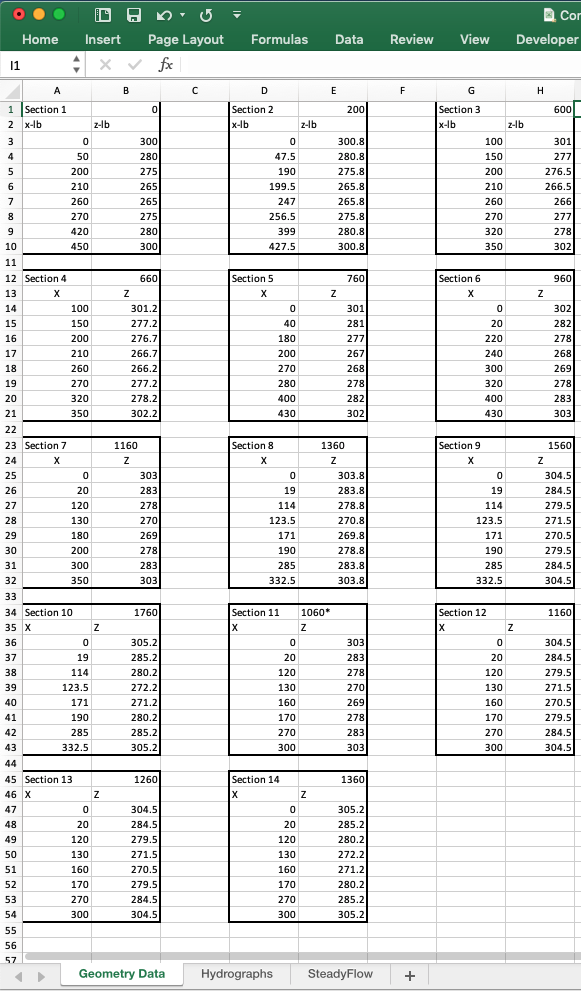
\includegraphics[height=5in]{cross-sections-table.png} 
   \caption{Tabular cross sections }
   \label{fig:cross-sections-table}
\end{figure}
Section 11 connects to the main channel between Section 6 and 7, and that is the meaning of the ``*'' symbol in the table.
The angle that the tributary forms with the main channel is about 60-degrees.
X-LB and Z-LB are distance and elevation relative to the left bank of each section. %--- Figure 2 is a plot of Section 3 for reference.

The road is cut into the surrounding grade so that the low chord of the bridge at the main channel is at elevation 290, and the roadway surface is at elevation 295 feet.  
\clearpage
Figure \ref{fig:steady-flow-conditions} is a table of steady flow conditions to consider. 

\begin{figure}[h!] %  figure placement: here, top, bottom, or page
   \centering
   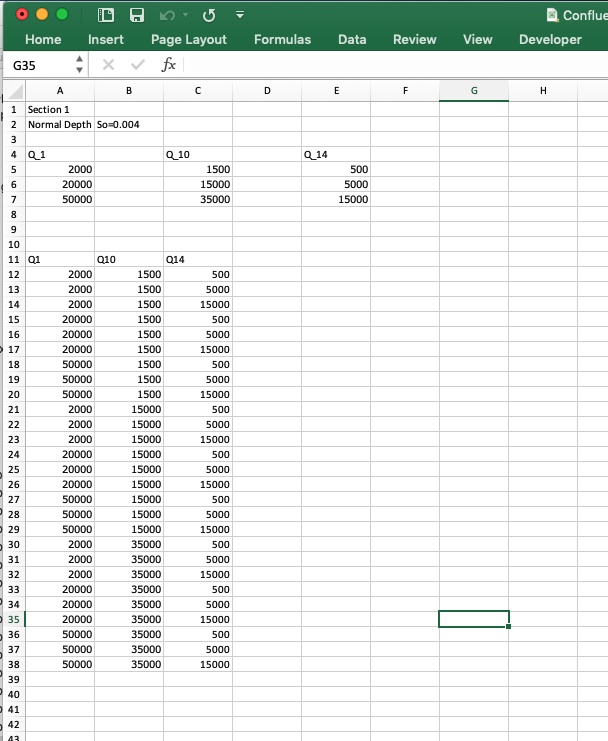
\includegraphics[height=5in]{steady-flow-conditions.png} 
   \caption{Steady flow conditions - various combinations}
   \label{fig:steady-flow-conditions}
\end{figure}
Determine if the current bridge low chord can accommodate the different flows. 
If flow cannot clear the low chord, treat the bridge as a large culvert and determine if the roadway surface is still passable (not flooded).

Repeat the analysis assuming the bridge abutments extend 100 feet into the left and right over-bank.
\clearpage
Figure \ref{fig:hydrographs-table} is a table of transient flow conditions to consider. 
\begin{figure}[h!] %  figure placement: here, top, bottom, or page
   \centering
   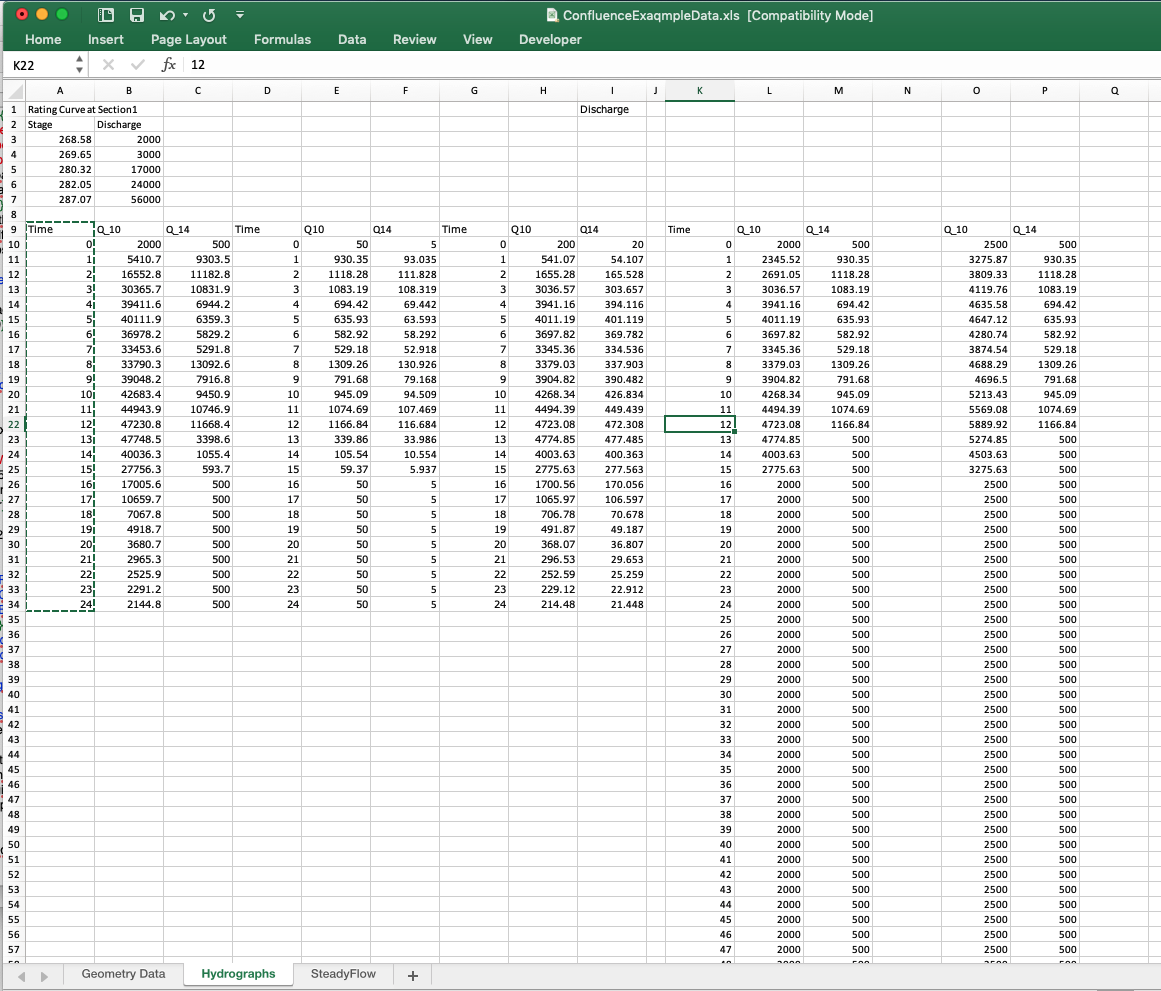
\includegraphics[height=5in]{hydrographs-table.png} 
   \caption{Transient flow conditions }
   \label{fig:hydrographs-table}
\end{figure}
\newline
Determine if the current bridge low chord can accommodate the different flows.  


If flow cannot clear the low chord, treat the bridge as a large culvert and determine if the roadway surface is still passable (not flooded).

Repeat the analysis assuming the bridge abutments extend 100 feet into the left and right over-bank.






\subsection{Appendix}

%%%%%%%%%%%%%%%%%%%%%%%%%%%%%%%%%%%%%%%

%%%%%%%%%%%%%%%%%%%%%%%%%%%%%%%%%%%%%%%%
%%%%% BIBLIOGRPAHY %%%%%%%%%%%%%%%%%%%%%%%%%%
%%%%%%%%%%%%%%%%%%%%%%%%%%%%%%%%%%%%%%%%
\begin{thebibliography}{}

%\bibitem[\protect\citeauthoryear{Christian and Griffiths}{Christian and Griffiths}{2016}]{Christian2016}
%Christian, B. and Griffiths, T. (2016).?
%\newblock Algorithms to Live By: The Computer Science of Human Decisions
%\newblock Henry Holt and Co.. Kindle Edition. 
\bibitem[\protect\citeauthoryear{Koutitas}{Koutitas}{1983}]{Koutitas1983}
Koutitas, C.G. (1983).
\newblock {\em Elements of Computational Hydraulics}.
\newblock Pentech Press, London 138p.
\newblock ISBN 0-7273-0503-4 

\bibitem[\protect\citeauthoryear{Roberson}{Roberson}{1988}]{Roberson1988}
Roberson, J A., Cassidy, J.J., and Chaudhry, M. H. (1988).
\newblock {\em Hydraulic Engineering}.
\newblock Houghton Mifflin Co., Boston, 662p.
\newblock ISBN 0-395-38123-1

\bibitem[\protect\citeauthoryear{Sturm}{Sturm}{2001}]{Sturm2001}
Sturm T.W (2001).
\newblock {\em Open Channel Hydraulics, 1ed.}.
\newblock McGraw-Hill, New York.

\bibitem[\protect\citeauthoryear{Cunge, et. al. }{Cunge, et. al.}{1980}]{Cunge1980}
Cunge, J.A., Holly, F.M., Verwey, A. (1980). 
\newblock Practical Aspects of Computational River Hydraulics.
\newblock Pittman Publishing Inc. , Boston, MA. pp. 7-50 

%\bibitem[\protect\citeauthoryear{Zheng and Bennett}{Zheng and Bennett}{1995}]{Zheng1995}
%Zheng, C. and Bennett, G. D. (1995).
%\newblock {\em Applied Contaminant Transport Modeling}.
%\newblock Van Nostrand Reinhold.

%
%\bibitem[Press(1986)]{Press1986}
%Press, W.H., Flannery, B.P., Teukolsky, S.A., Vettering, W. T. 1986, Numerical Recipes:\textsl{The Art of Scientific Computing}.  Cambridge University Press, London.  818p.
%
%\bibitem[Gill(1981)]{Gill1981}
%Gill, P.E., Murray, W, Wright, M. H., 1981. Practical Optimization.  Academic Press, San Diego. 401p.

%\bibitem[Wiki(1999)]{Wiki(1999)}
%Wikipedia discussion of Newton's method.
%\url{http://en.wikipedia.org/wiki/Newton's_method}.
%
%\bibitem[Wiki(2000)]{Wiki(2000)}
%Wikipedia discussion of matrix inversion.
%\url{http://en.wikipedia.org/wiki/Invertible_matrix}.

%\bibitem[\protect\citeauthoryear{Christian and Griffiths}{Christian and Griffiths}{2016}]{Christian2016}
%Christian, B. and Griffiths, T. (2016).
%\newblock Algorithms to Live By: The Computer Science of Human Decisions
%\newblock Henry Holt and Co.. Kindle Edition. 

%\bibitem[\protect\citeauthoryear{Chin}{Chin}{2006}]{chin2006}
%Chin, D.~A. (2006).
%\newblock {\em Water-Resources Engineering}.
%\newblock Prentice Hall.
%
%\bibitem[\protect\citeauthoryear{Haman and Brameller}{Haman and Brameller}{1971}]{Haman1971}
%Haman YM, Brameller A. (1971)
%\newblock{Hybrid method for the solution of piping networks}. 
%\newblock{Proc IEEE 1971;118(11):1607-12}.
%
%\bibitem[\protect\citeauthoryear{Gironas, Roesner, and Davis}{Gironas
%  et~al.}{2009}]{gironas2009}
%Gironas, J., L.~A. Roesner, and J.~Davis (2009).
%\newblock {Storm Water Management Model} applications manual.
%\newblock Technical Report EPA/600/R-09/077, U.S. Environmental Protection
%  Agency, National Risk Management Research Laboratory Cincinnati, OH 45268.
%
%\bibitem[\protect\citeauthoryear{NCEES}{NCEES}{2008}]{ncees2008}
%NCEES (2008).
%\newblock {\em Fundamentals of Engineering Supplied Reference Handbook\/} (8th
%  ed.).
%\newblock 280 Seneca Creek Road, Clemson, SC 29631: National Council of
%  Examiners for Engineering and Surveying {ISBN 978-1-932613-37-7}.
%
%\bibitem[\protect\citeauthoryear{Rossman}{Rossman}{2000}]{rossman2000}
%Rossman, L. (2000).
%\newblock {EPANET 2} users manual.
%\newblock Technical Report EPA/600/R-00/057, U.S. Environmental Protection
%  Agency, National Risk Management Research Laboratory Cincinnati, OH 45268.
%
%\bibitem[\protect\citeauthoryear{Rossman}{Rossman}{2009}]{rossman2009}
%Rossman, L. (2009).
%\newblock {Storm Water Management Model} user's manual version 5.0.
%\newblock Technical Report EPA/600/R-05/040, U.S. Environmental Protection
%  Agency, National Risk Management Research Laboratory Cincinnati, OH 45268.



%\bibitem[Asquith(1998)]{Asquith1998}
%Asquith, W.H., 1998, Depth-duration frequency of precipitation for Texas: U.S. Geological Survey Water-Resources Investigations Report 98�4044, 107 p., \url{http://pubs.usgs.gov/wri/wri98-4044/}.
%
%\bibitem[Asquith and Roussel(2004)]{AR2004}
%Asquith, W.H., and Roussel, M.C., 2004, Atlas of depth-duration frequency of precipitation annual maxima for Texas: U.S. Geological Survey Scientific Investigations Report 2004�5041, 106 p.
%
%\bibitem[Chow and others(1988)]{Chow1988}
%Chow, V.T., Maidment, D.R., Mays, L.W., 1988, Applied Hydrology: New York,
%McGraw-Hill.
%
%\bibitem[Hann and others(1994)]{Hann1994}
%Haan, C.T., Barfield, B.J., and Hayes, J.C., 1994, Design Hydrology and Sedimentology for Small Catchments: San Diego, Academic Press.
%
%\bibitem[McCuen and others(2002)]{McCuen2002}
%McCuen, R.H., Johnson, P.A., and Ragan, R.M., 2002, Hydraulic Design Series
%No. 2�Highway Hydrology, 2nd ed., October 2002: U.S. Department of Transportation, Federal Highway Administration, National Highway Institute, FHWA Pub. No. NHI-02-001, accessed on Sept. 26, 2014 at \url{http://www.fhwa.dot.gov/ engineering/ hydraulics/library_arc.cfm?pub_number=2&id=6  and http://isddc.dot.gov/OLPFiles/FHWA/013248.pdf}.
%%
%\bibitem[Texas Department of Transportation(2014)]{TxDOT2014}
%Texas Department of Transportation, 2014, Hydraulic Design Manual, rev. May
%2014: Texas Department of Transportation, accessed on September 26, 2014 at \url{http:
%//onlinemanuals.txdot.gov/txdotmanuals/hyd/hyd.pdf}. 


%\bibitem[Asquith and Slade(1997)]{AS1997}
%Asquith, W.H., and Slade, R.M., 1997, Regional equations for estimation of peak-streamflow frequency for natural basins in Texas: U.S. Geological Survey Water Resources Investigations Report 96--4307, \url{http://pubs.usgs.gov/wri/wri964307/}.
%
%\bibitem[Asquith, and Roussel (2009)]{AR2009}
%Asquith, W.H., and Roussel, M. S., 2009, Regression equations for estimation of annual peak-streamflow frequency for undeveloped watershed in Texas using an L-moment-based, PRESS-minimized, residual adjusted approach. U.S. Geological Survey Scientific Investigations Report 2009--5087.
%
%\bibitem[Asquith, Herrmann, and Cleveland(2013)]{AsquithQVGAM2013}
%Asquith, W.H., Herrmann, G.R., and Cleveland, T.G., 2013, Use of generalized additive modeling for regionalization of a discharge measurement database in Texas. Journal of Hydrologic Engineering, American Society of Civil Engineers, \textsl{in press}
%%
%\bibitem[Gordon and others(2004)]{Gordon2004}
%Gordon, N.D., T.A. McMahon, B.L. Finlayson, C.J. Gippel, R.J. Nathan, 2004,
%Stream Hydrology: An Introduction for Ecologists (second edition). John Wiley, The Atrium, Southern Gate, Chichester, West Sussex PO19 8SQ,
%England, 429~p.

%\bibitem[\protect\citeauthoryear{Chin}{Chin}{2006}]{chin2006}
%Chin, D.~A. (2006).
%\newblock {\em Water-Resources Engineering}.
%\newblock Prentice Hall.
%
%\bibitem[\protect\citeauthoryear{Gironas, Roesner, and Davis}{Gironas
%  et~al.}{2009}]{gironas2009}
%Gironas, J., L.~A. Roesner, and J.~Davis (2009).
%\newblock {Storm Water Management Model} applications manual.
%\newblock Technical Report EPA/600/R-09/077, U.S. Environmental Protection
%  Agency, National Risk Management Research Laboratory Cincinnati, OH 45268.
%
%\bibitem[\protect\citeauthoryear{NCEES}{NCEES}{2008}]{ncees2008}
%NCEES (2008).
%\newblock {\em Fundamentals of Engineering Supplied Reference Handbook\/} (8th
%  ed.).
%\newblock 280 Seneca Creek Road, Clemson, SC 29631: National Council of
%  Examiners for Engineering and Surveying {ISBN 978-1-932613-37-7}.
%
%\bibitem[\protect\citeauthoryear{Rossman}{Rossman}{2000}]{rossman2000}
%Rossman, L. (2000).
%\newblock {EPANET 2} users manual.
%\newblock Technical Report EPA/600/R-00/057, U.S. Environmental Protection
%  Agency, National Risk Management Research Laboratory Cincinnati, OH 45268.
%
%\bibitem[\protect\citeauthoryear{Rossman}{Rossman}{2009}]{rossman2009}
%Rossman, L. (2009).
%\newblock {Storm Water Management Model} user's manual version 5.0.
%\newblock Technical Report EPA/600/R-05/040, U.S. Environmental Protection
%  Agency, National Risk Management Research Laboratory Cincinnati, OH 45268.

\end{thebibliography}

\end{document}  
Meriam and Kraige, 1997.  Engineering Mechanics - Vol. 1. J. Wiley & Sons, New York. (Simple Numerical Integration Formulas)

Cornell, G. 1993.  Visual Basic 3 for Windows Handbook.  McGraw Hill , New York.

%At this point we will want to convert the string into a float and assign the values element-by-element to the matrix \texttt{amatrix}.
%To do so I am using a very POP (procedural oriented programming) structure to make the assignment -- there is surely better ways to accomplish this task, but for the time being this will suffice.
%
%\begin{verbatim}
%# convert data type to float, populate amatrix
%for i in range(0,rowNumA,1):
%    for j in range(0,len(any_matrix[0])):
%        amatrix.append(float(any_matrix[i][j]))
%\end{verbatim}

%The above portion of the code uses two for loops, one to count ``rows'' and the other to count columns.  Again the \texttt{.append} method is employed, but this time on the  \texttt{amatrix} list, and the contents of \texttt{any\_matrix}, indexed by the row-column subscript, are converted to a float before the actual appending to the list.

%A slice is a lot like the integration panels.  The left edge of the slice looks to the right, the right edge looks to the left.   
%Figure \ref{fig:SliceSchemeOne} is a graphical depiction of the slice concept on a list (in this case the \texttt{matrix} list).
%
%\begin{figure}[h!] %  figure placement: here, top, bottom, or page
%   \centering
%   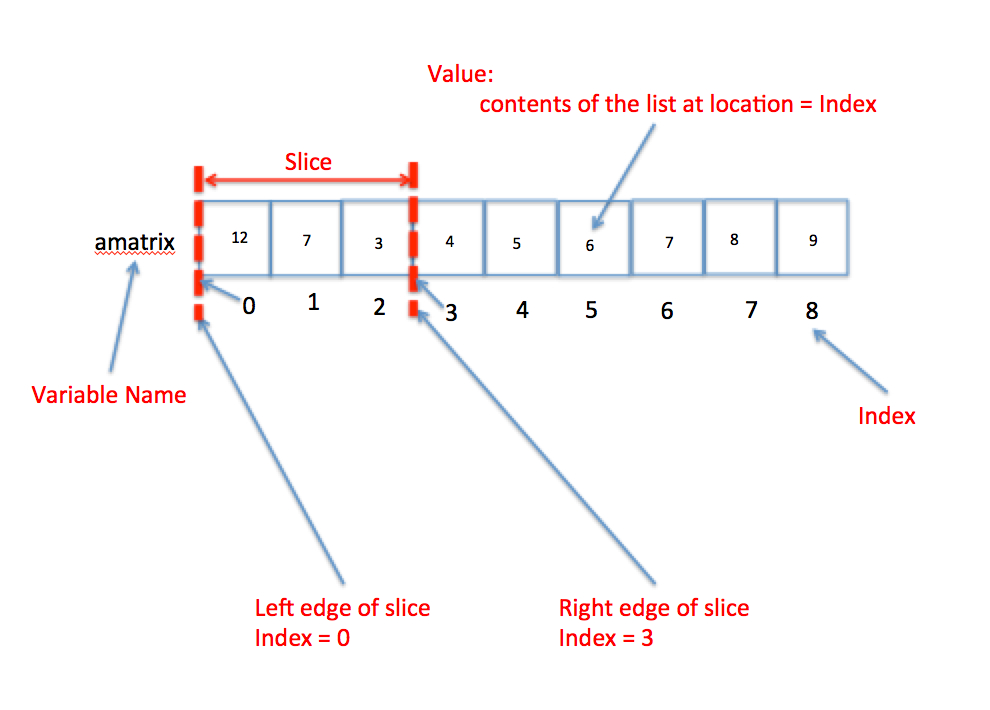
\includegraphics[width=6in]{./Matrix/SliceSchemeOne.jpg} 
%   \caption{Concept of slice from a list.}
%   \label{fig:SliceSchemeOne}
%\end{figure}
%
%So the index to the right of the left edge is the beginning of the slice, the index to the right of the right edge is the index of the end of the slice.  
%
%Alternatively we can simply say that Python addresses an index list from start to end, but does not actually get the end value, instead only end-1.  It's weird, but it is how the author of Python created the language.   FORTRAN has a similar weirdness in that it starts at 1 (rather than zero) for its counting scheme.
%
%Figure \ref{fig:SlicesAndMatrix} is a schematic of how slices and the row column structure of a matrix are conceptualized.   As far as the computer is concerned, a matrix is just a long list and we (humans) are the fools who invented this whole row column thing.   I find that if I think of the matrix as a vector with Z-folds at the column ends, I can deconstruct the single list into a set of lists, now indexed by row and column (just like I was taught in linear algebra forever ago).
%
%\begin{figure}[h!] %  figure placement: here, top, bottom, or page
%   \centering
%   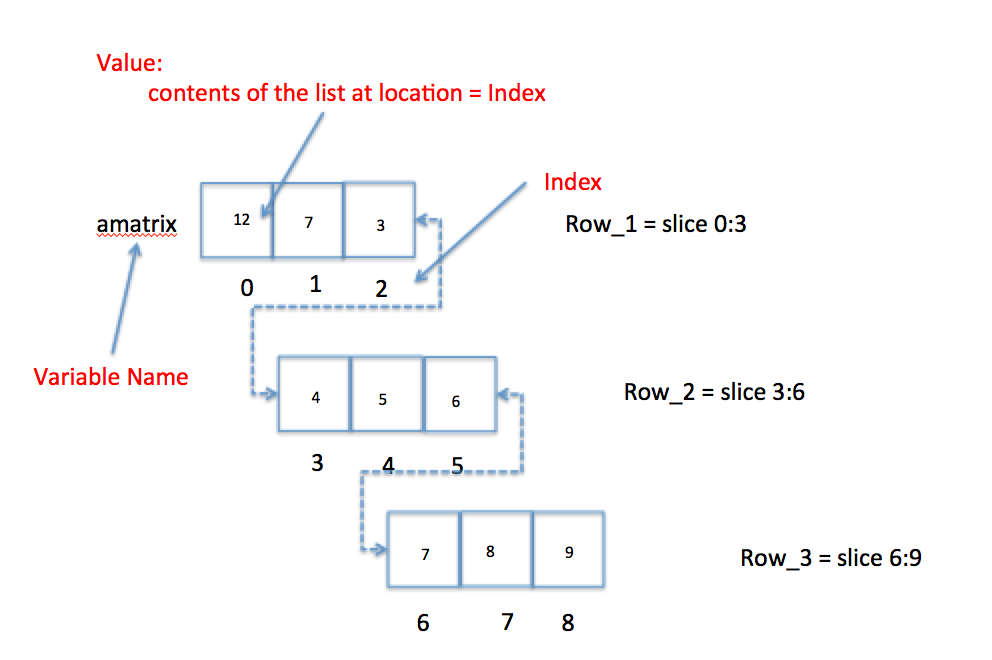
\includegraphics[width=6in]{./Matrix/SlicesAndMatrix.jpg} 
%   \caption{A conceptual diagram of slices and matrix relationships.  Each slice becomes a row.  We refer to an element by its row column index e.g. \texttt{amatrix[row][col]}. }
%   \label{fig:SlicesAndMatrix}
%\end{figure}

But this simply won't work because lists while they can contain floats, are not themselves floats -- the are lists.  So the above code which would be super natural in FORTRAN, C++, BASIC, ALGOL, PASCAL, RUBY, is useless in Python.  

However the following works quite nicely
\begin{verbatim}
amatrix[:] = [value * MyScalar for value in amatrix]
\end{verbatim}

